\documentclass[border=2pt]{standalone}
\usepackage{pgfplots}
\pgfplotsset{compat=1.18}
\begin{document}
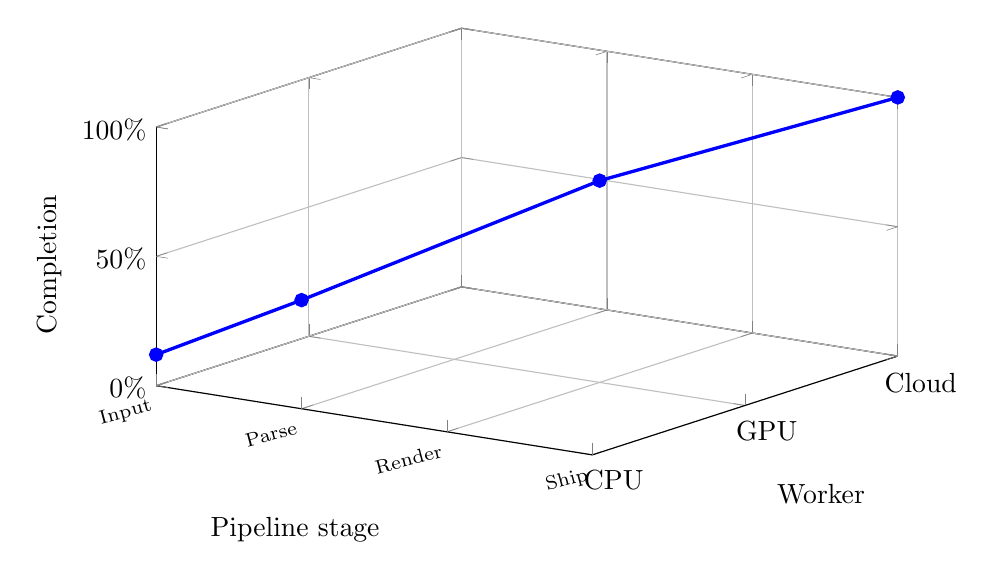
\begin{tikzpicture}
  \begin{axis}[
    width=11cm,
    height=7cm,
    view={35}{25},
    xmin=0,
    xmax=3,
    ymin=0,
    ymax=2,
    zmin=0,
    zmax=100,
    xtick={0,1,2,3},
    xticklabels={Input,Parse,Render,Ship},
    ytick={0,1,2},
    yticklabels={CPU,GPU,Cloud},
    ztick={0,50,100},
    zticklabel={\pgfmathprintnumber{\tick}\%},
    x tick label style={rotate=15,anchor=north east,font=\scriptsize},
    grid=major,
    xlabel={Pipeline stage},
    ylabel={Worker},
    zlabel={Completion}
  ]
    \addplot3[blue,very thick,mark=*] coordinates {
      (0,0,12) (1,0,42) (2,1,78) (3,2,100)
    };
  \end{axis}
\end{tikzpicture}
\end{document}
